%+------------------------------------------------------------------------+
%| Diagram: Configuration spaces of continuum media
%| Author: Antonio miti
%| 
%+------------------------------------------------------------------------+


\documentclass[border=5pt]{standalone}
\usepackage{tikz}
\usepackage{mathtools}
\usepackage{amsfonts}
\usetikzlibrary{decorations.pathmorphing}



\begin{document}
	\begin{minipage}[t]{\linewidth}
				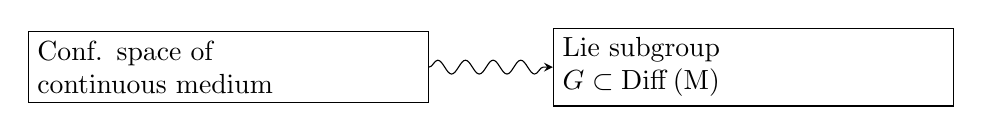
\begin{tikzpicture}[
					text width=0.4\linewidth,
					node distance=0.55\linewidth,
					]
					\node [rectangle,draw] (lhs) {Conf. space of\\ continuous medium};
					\node [rectangle,draw,right of=lhs] (rhs) {Lie subgroup \\$G \subset \rm{Diff}\,(M)$};
					\draw[-stealth,decorate,decoration={snake}] (lhs) -- (rhs);
				\end{tikzpicture}
		
				Examples:\\
				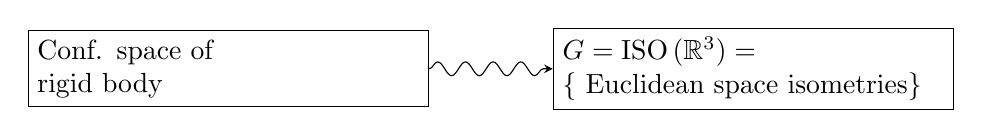
\begin{tikzpicture}[
					text width=0.4\linewidth,
					node distance=0.55\linewidth,
					]
					\node [rectangle,draw] (lhs) {Conf. space of\\ rigid body};
					\node [rectangle,draw,right of=lhs] (rhs) {$G=\rm{ISO}\,(\mathbb{R}^3)=$\\ $\{$
						Euclidean space isometries$\}$};
					\draw[-stealth,decorate,decoration={snake}] (lhs) -- (rhs);
				\end{tikzpicture}
				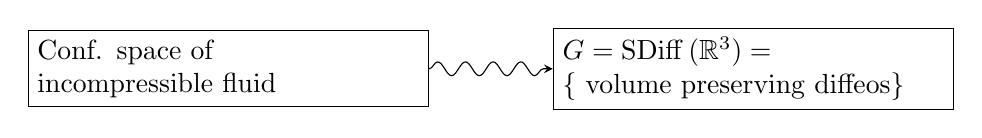
\begin{tikzpicture}[
					text width=0.4\linewidth,
					node distance=0.55\linewidth,
					]
					\node [rectangle,draw] (lhs) {Conf. space of\\ incompressible fluid};
					\node [rectangle,draw,right of=lhs] (rhs) {$G= \rm{SDiff}\,(\mathbb{R}^3)=$\\ $\{$
						volume preserving diffeos$\}$};
					\draw[-stealth,decorate,decoration={snake}] (lhs) -- (rhs);
				\end{tikzpicture}	
	\end{minipage}
\end{document}

	